%----------------------------------------------------------------------------------------
%	PACKAGES AND OTHER DOCUMENT CONFIGURATIONS
%----------------------------------------------------------------------------------------
% !TeX TS-program = pdflatexmk

\documentclass[a4paper,11pt]{scrreprt}
\usepackage[hscale=0.69,vscale=0.79,heightrounded,includehead]{geometry}
%\pagestyle{headings}
\usepackage{fancyvrb}
\usepackage[usenames,dvipsnames]{xcolor}
\usepackage{soul}
\usepackage{wrapfig}
\usepackage[english]{babel}
\usepackage{graphicx}
\graphicspath{ {../graphics/} }
\usepackage{floatrow}
\usepackage{babel}
\usepackage{csquotes}
\usepackage{caption}
\usepackage{subcaption}
\usepackage[T1]{fontenc}
\usepackage{float}
\usepackage[backend=biber]{biblatex}
\addbibresource{references.bib}
\usepackage{epstopdf}
\usepackage{hyperref}
\usepackage{listings}
\usepackage{color}
\newcommand{\HRule}{\rule{\linewidth}{0.5mm}}
\definecolor{dkgreen}{rgb}{0,0.6,0}
\definecolor{gray}{rgb}{0.5,0.5,0.5}
\definecolor{mauve}{rgb}{0.58,0,0.82}
\usepackage{amssymb,amsmath}
\usepackage{abstract}

\addtokomafont{chapterprefix}{\raggedleft}
\renewcommand*{\chapterformat}{%
\mbox{\chapappifchapterprefix{\nobreakspace}%
\scalebox{5}{\color{gray}\thechapter\autodot}\enskip}%
}


%----------------------------------------------------------------------------------------
%	BEGIN & TABLE OF CONTENTS
%----------------------------------------------------------------------------------------
\begin{document}

\title{Realtime Classification Engine}
\subtitle{Msc Intelligent Systems Dissertation}
\author{Andrew Haines\\
	University of Sussex\\
	\texttt{ajh21@sussex.ac.uk}}

\date{\today}
\maketitle

\begin{abstract}
With the invent of processing platforms that allow for cheap, commodity hardware to run horizontally distributed applications at unprecedented scale, never before have we seen such an explosion of data collection and processing. Because of this abundance of processing power and ever cheaper storage costs, there is a growing trend to capture and collect events, limited only by what can be instrumented and regardless of an immediate requirement. These persisted events sit dormant in data centers waiting for their vast coffers to be harvested for valuable insights and application. Many of the algorithms and developments that have arisen out of this have relied on the fact that even though such sporadically collected data is noisy, with enough of it, the law of large numbers suggests that signals can still emerge and be fed into a new breed of intelligent systems\cite{bigdata}. The problem with this approach is that, although tractable to large institutions and organizations, smaller, more modest individuals will not have the infrastructure or financing to support such data collection even though their reach is enough to warrant its need. Tech startups in particular face this problem all the time balancing the business insights and intelligent feature sets they provide to their customers at the trade off of vast equity deals in seeding rounds.\\

In this project we attempt to design and build a closed domain application that runs at 'big data' scale but on a single machine instance. The closed domain of the application is one of a classifier that, given an entity or event expressed in a feature space, it will recommend suggested classes based on a continuous stream of online data input. The ideas and concepts that semantically define this recommender are nothing new but its implementation and structure is novel and works by making extensive use of modern computer architecture to process events far quicker than traditional techniques.

\end{abstract}

\tableofcontents

\chapter{Background}
More and more large institutions these days rely on the analysis of vast quantities of data to inform business decisions and provide performance feedback. From tracking the performance of advertising campaigns, constructing weather models, and powering recommendation engines, Big Data processing is rapidly becoming the cornerstone of the online technology industry. Large companies such as Google and IBM spend hundreds of millions of pounds in capex to construct and maintain the processing systems required to mine this data. These systems are typically generic platforms developed across many thousands of machines and delivered company-wide to cater for all business units in the organization. Resources such as storage and compute time are then shared across all applications of the organisation. To accommodate this, fully distributed but virtualised operating systems have been developed that allows applications, built upon generic frameworks, to be deployed and scheduled on these 'grid' infrastructures of machines and networking topologies.\\

\section{Big Data Processing Paradigms}
The current state of the art in these distributed frameworks fall primarily into two distinct camps.
\subsection{Batch Processing}
The first type of framework is one that follows a batch processing methodology. The concept is that data is persisted onto a distributed file system in near raw form. Processing then operates on the data either as a one off task for insight analysis or bootstrapping purposes or, at periodic intervals that produce transformed data that can be used in downstream processes. To illustrate this, consider a possible implementation of a 'trending now' feature on a large web property's home page, used to inform users of what is currently popular on the domain at that time. \\

To determine this, the web property instruments all interactions with various content on its systems. This could be tweets sent from a mobile device app or news articles clicked on via a user's web browser - all events are logged to a central analytics system with a pre defined payload. This payload could contain information about the user\footnote{gender, age, personal preferences, etc}, the local time the event occurred at, information about the device, the content UUID interacted with... the tuple of data that could be chosen is endless. The analytics servers then typically place the event, via a messaging system onto the distributed file system \footnote{This file system is distributed in the sense that the data actually sits on multiple machines possibly  in geo graphically diverse data centers but appear as if it is one contiguous structure of files.} in a '\texttt{rawevents-YYYYMMDDHH-xxxx}' series of files. A scheduled task then runs every hour that consumes these latest files, extracts named entities from them and creates a histogram of their occurrences. The named entities are then ranked according to the histogram's frequency and the top x results are persisted into a '\texttt{trending-now-YYYYMMDDHH}' timestamped file. This comparatively tiny file is then sent to all the client facing webservers and powers the last hour's 'trending now' list.\\

Using the batch approach enables the data to be processed 'offline' in the sense that data is processed some time after the events have occurred.  This has a number of advantages over the cost of not being real time. Firstly, the programming concepts can be far easy to implement. Consider the calculation of a median value of a vast list of numerical objects. Using batch you would simply sort the list and pick the middle one as you have all the data for that given hour available. Indeed, if you choose to not remove the intermediate '\texttt{'rawevents'} files then larger periods can be scaled up by simply increased the file ranges. Handling in the event of error is also far easier as processing can easily be rerun. The other downside is that the demand on storage capacity is huge but, given the growing trend to capture all data and archive it for later insights, this tends to already be available.\\

There are 2 main concepts within batch processing that allow it to structure the control flow of the application.

\subsubsection{Map Reduce}
This technique is an adaptation of an old functional programming paradigm where by two phases of computation are established - the map phase and the reduce phase. Google took this paradigm and ported it to a distributed setting in 2004\cite{mapreduce}. The general idea is that during the map task, execution is moved to where the data is rather then data being moved to whether the executable code lies. The reason in the big data setting should be obvious as the IO costs involved in transporting vast quantities of data to executor machines is fair costlier and time consuming then moving a small executable to each of the machine that store the event files. Such machines are referred to as data nodes. Execution in the map phase then runs on the data nodes and is used to filter, transform and assign special keys to each record that this data node holds. The output, being typically alot smaller, 'shuffled' to reducer nodes which may (some IO costs) or may not (no costs incurred) be on different machines before finally being sorted by the special keys assigned during mapping. This allows all items assigned to a particular key to be available on a single reducer. In the case of the trending now example, this would equate to each instance of a named entity being sent to a single reducer so that it's component of the histogram - its particular count - can be computed (see Figure \ref{fig:MapReduceEx}). In 2011 Yahoo open sourced the HadoopMR\autocite{hadoopMR} module that forms part of the hadoop operating system.\\

\begin{figure}[h]
\centering
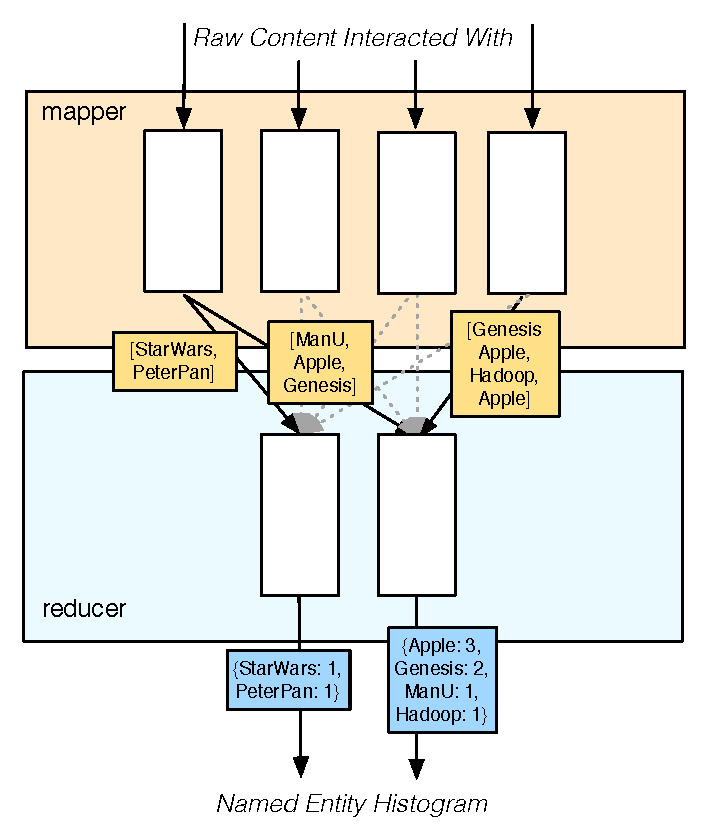
\includegraphics[scale=0.7] {MapReduceEx.pdf}
\caption{MapReduce Trending Now Example. For Brevity only 2 mappers are shown. The inputs to the process are the raw content data and the mappers determine which named entities are present. These are then keyed on the textual representation of the entity and all entities of the same name are sent to a single reducer. The output is then a frequency count of all named entities}
\label{fig:MapReduceEx}
\end{figure}

The problem with this approach is that, although it scales well when the distribution of the keys is uniform, in the face of skew in the key set, this bias is propaged down to the reducer load and can mean that a small number of machines can do the majority of the work. Also, as we have seen from the trending now example, the calculation of the distribution of terms is only one part of the entire process. It was assumed here that the entities of all the content that was interacted with had been previously computed. To do this using Map Reduce we would need another set of MR tasks that would extract the content from the raw events, normally only defined by the UUID, prior to the task described. The output is also just the raw counts, we would need a further step to then sort the entities by their counts and only persist the top x. This illustrates what typically happens with complicated MR applications in that a number of sub tasks of mapping and reducing have to occur with intermediate temporary files coordinating the data flow between them. This can be both limiting in how a application is structured and also inefficient due to unnecessary persistence of these temporary files. To solve this the DAG approach was devised:

\subsubsection{DAG}

\begin{figure}[H]
\centering
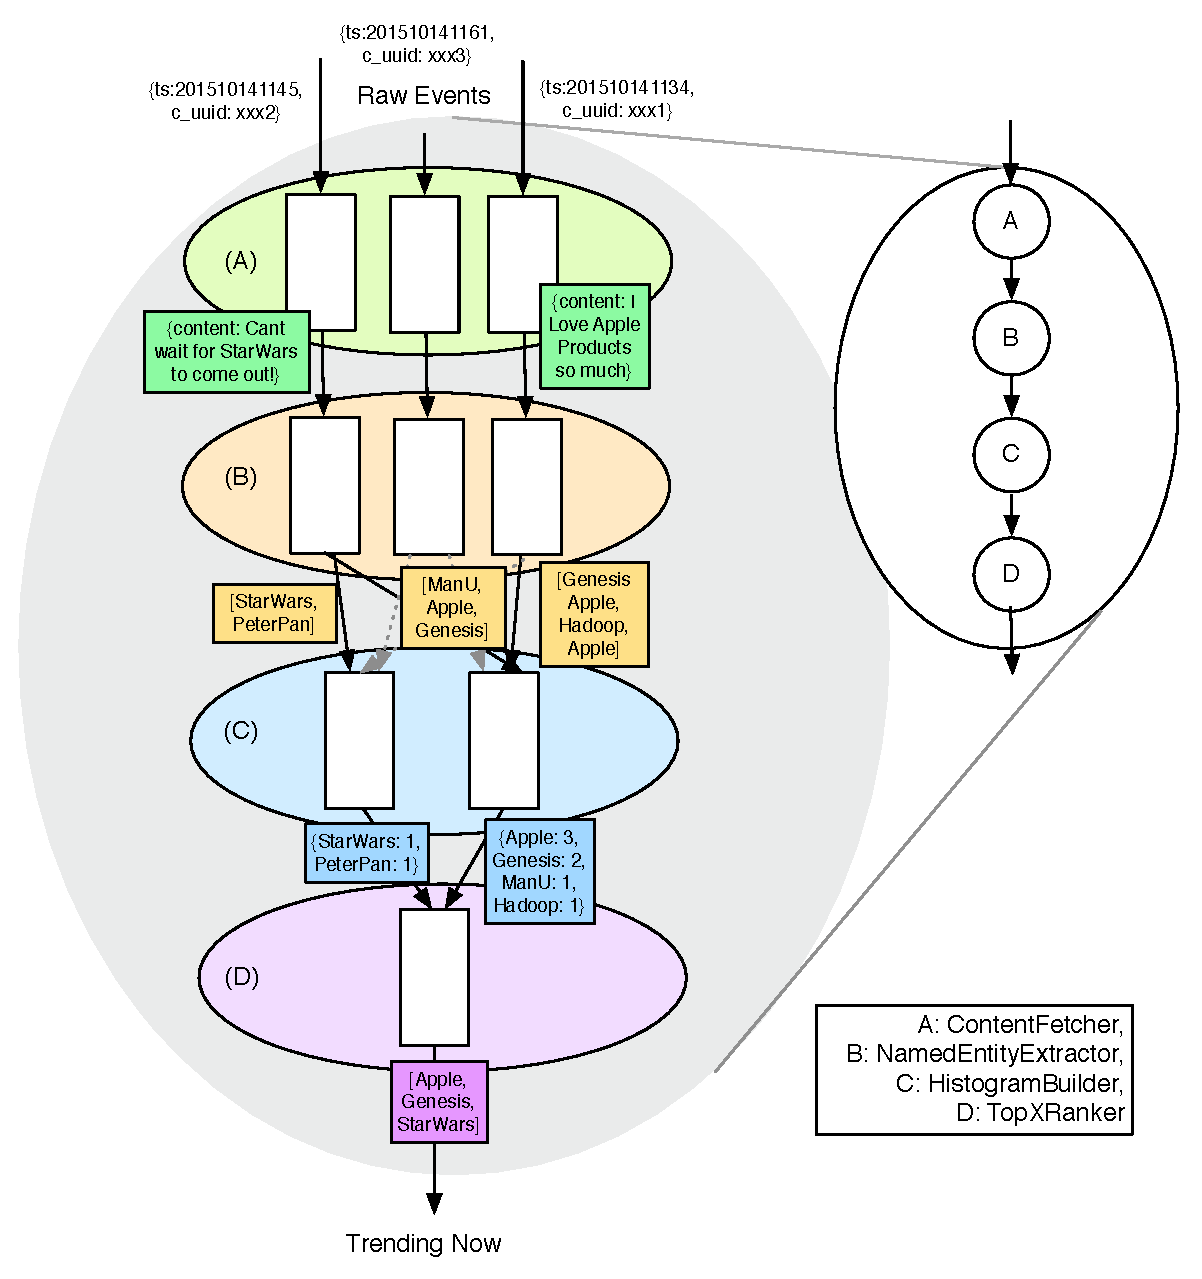
\includegraphics[scale=0.65] {DAG.pdf}
\caption{DAG Trending Now Example. In this example the entire application is shown, not just the histogram building. Data flows through the graph along the edges to the nodes. In this example, the DAG framework is able to determine that both the content fetcher and the name entity extractor need never move any data around and so the computation actually happens on the same nodes without ever having to write to disk}
\label{fig:DAGEx}
\end{figure}

The Directed Acyclic Graph\cite{dryad, spark-paper} approach tackles the deficiencies of MR by defining a graph of tasks that have to be executed concurrently. Nodes in the graph are sub tasks that need to be performed and the edges are data flows between them. Nodes are distributed as in MR by moving them to where the data is but there exists far more flexibility in how an execution flow can be maintained and structured. In the trending now example, a node can exist for extracting the entities of the file, where the determined entities are then fed into the distribution calculation node to obtain counts prior to another node that then filters out the x largest entities (see Figure \ref{fig:DAGEx}). Libraries such as tez\cite{tez-site} and spark\cite{spark-site} are two popular frameworks currently gaining traction in the industry.

\subsection{Stream processing}
One of the big problems with batch processing is that it is not real time. For most applications this isn't too much of a draw back but imagine budget caps on an advertiser spend. Waiting for the next hour's processing window to cut off an advertisers supply could be extremely costly. Assuming that processing never overruns\footnote{There is overhead with starting up distributed tasks that can easily make stall resource allocation and cause SLA's to be missed}, near realtime updates could be possible by reducing the processing window of the batch to a few minutes to help mitigate this issue but this isn't going to help a nuclear cooling processor from reacting to a sudden over heating. Stream processing provides a solution to this by processing events in a stream manner as they enter the system and distributed across a cluster of nodes. This means that events are processed, for the most part, either directly from the network bus or in a temporarily buffer, but never needing to be saved on the distributed file system. Processing is structured as a topology using concepts such as spouts and bolts to represent the data flow and processing respectively. In the trending now example, processing occurs in a very similar manner to that of the DAG approach. The difference being of course that at no point does a node get to see anything other than the current event. This is fine in our trending now example until we get to the ranking stage. \\

Choices have to be made in streaming about concepts like where an accumulating histogram is stored and for how long does it persist for? There is no point in keeping the histogram for all time as this defeats the purpose of the trending \textbf{\textit{\underline{now}}}. One option would be to reset every hour, assuming the behavior of the batch processing methodology - except that it wouldn't. A few seconds after the reset and there may not be enough data seen in the histogram to make accurate predictions meaning that periods just after each reset are inherently noise as the law of large numbers does not hold. Another approach would be a rolling window but this means that you need to keep all events in memory for each window. The larger the window the more likely to exhaust memory whilst smaller windows may not capture enough data. Also consider the median calculation mentioned previously. Without access to all the events, online versions such as a TDigest\cite{tdigest} need to be used which are far harder to implement and understand. Not only is stream based programming a lot harder but they are also extremely sensitive to the throughput coming and what can actually be processed. If your cluster is not large enough to process the influx of events coming into the system, then events are either dropped or buffered, reducing it's real time nature.\\

Obviously the upside of the stream approach, other than it's realtime operating behavior, is that it's also super fast as IO is reduced to bare minimum. Apache Storm\cite{storm-site}\footnote{a commonly used distributed stream processing framework open sourced from Twitter\cite{storm-twitter}. Apache Spark also offers a streaming mode but underneath the hood this is really a micro batch mode to approximate real time\cite{spark-streaming-paper}} claims to be able to process 1M events a second using just a 10 node cluster\footnote{It is worth mentioning that the author's experience of such throughput requires slightly more nodes in a real setting}. Furthermore, if storage capacity is deemed a premium, then this approach can allow big data processing to function without the need of a distributed file system. 

\subsection{High Throughput Systems}
On the other side of the technology spectrum, high throughput processing used in real time exchanges such as those within financial and scientific industries, are able to process huge streams of data but instead of scaling horizontally by adding more machines into a cluster, a single workhouse instance is used with multiple CPUs, huge memory addresses and dedicated transport buses that coordinate the data between. These are concurrent systems that are considered to scale vertically because obtaining more processing power and memory involves the reconfiguration of the instance itself by adding better CPU's or memory modules. These bespoke systems execute code that is specifically tailored to the underlying hardware which makes them incredibly efficient and able to outperform similar speced Hadoop or Storm clusters. Although typically favoring CPU bound tasks, these so called 'supercomputers' can still process vast amounts of data.
\begin{figure}[h!]

\centering
\caption{An example of a 2 core event driven data flow using disruptors to coordinate the transfer of events}
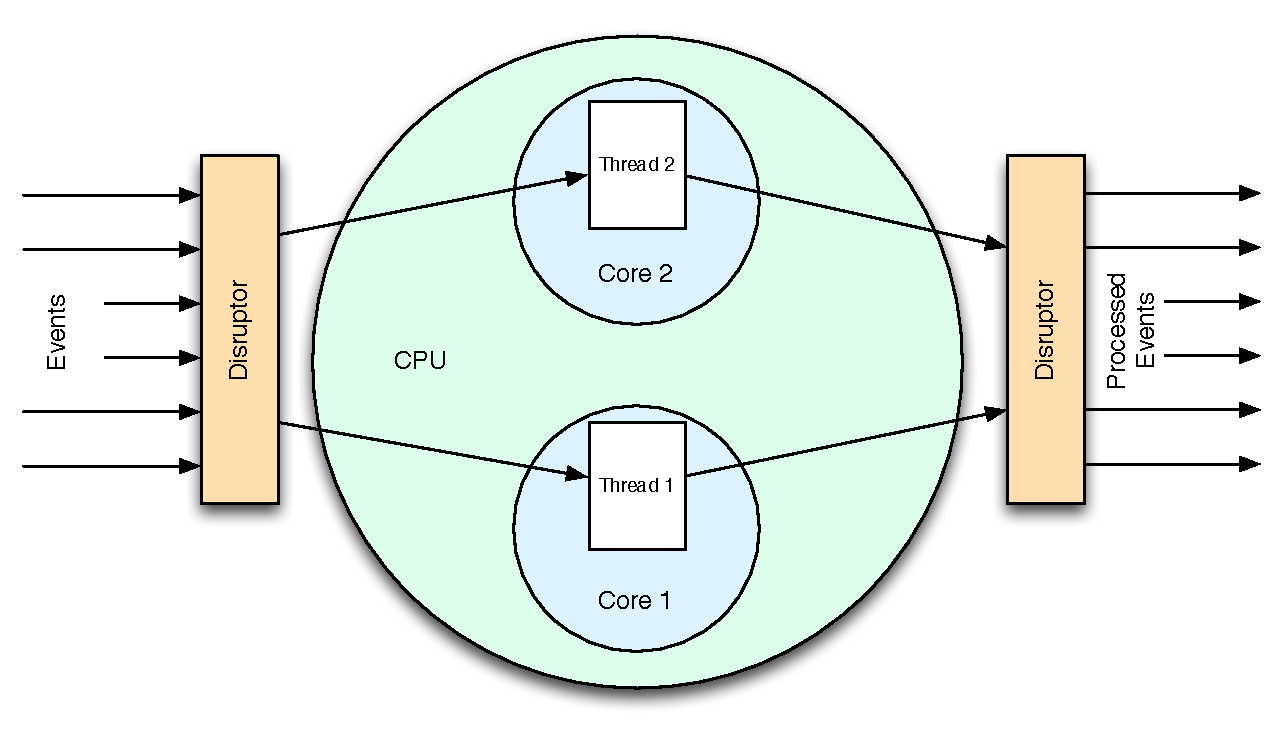
\includegraphics[scale=0.65] {disruptor-ex.pdf}
\label{fig:disruptor-ex}
\end{figure}

Further to this, the LMAX exchange in 2011 released a high throughput processing toolkit that borrowed from similar principles of software and hardware cooperation. Using techniques borrowed from synergising hardware and software, this toolkit is capable of supporting 25M events a second on a single commodity instance\cite{disruptor-paper}. This is not actual computational work mind, just moving events from one conceptual area of a program to another under concurrently safe conditions. None-the-less, achieving such high rates of transfer in in a thread safe manner is still highly impressive. It accomplishes this by using lock-less queues known as \textit{disruptors} that exploit a perfect \textit{mechanical sympathy} between high level programming paradigms and the under lying hardware infrastructure. The basic idea is that disruptors can act as brokers for events, passing them to different areas of code that may or may not be on different threads. This enables event driven design where threads are only used to pin execution to a particular CPU core\cite{processor-affinity}. These long running threads then can operate on the events from the disruptor using the single writer paradigm which ensures that write contention is no longer a concern and only care about visibility to other reader threads need be considered(see \ref{fig:disruptor-ex}). The worker threads can then pass events through the system without costly synchronisation and thread context switching.

Disruptors obtain their ultra fast design by utilising cache line structures and memory barriers present on modern cpus. They are essentially queues implemented in ring buffers where the majority of access is completely unsynchronised - care only be taken to ensure that threads have visibility of events on the buffer. Using a volatile pointer to the index of the buffer, as long as all event processors do not read past the writer position, no locking is required. 
\floatsetup[figure]{capposition=beside,capbesideposition={top,right}}
\begin{figure}[h]
\centering
\caption{The ring buffer at the heart of the disruptor design. For clarity the writer and reader positions are illustrated as if they are concerns of the Producer and EventProcessor respectively - however this is not the case in implementation as the ring buffer owns the pointers in order to ensure writerPos < readerPos}
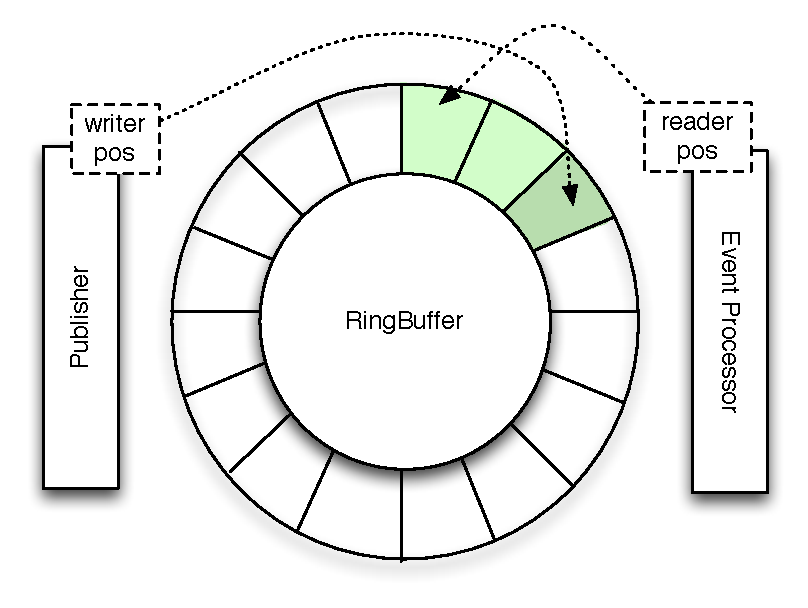
\includegraphics[scale=0.65] {ringbuffer.pdf}
\label{fig:ringbuffer}
\end{figure}

In the one scenario where the reader and writer are pointing to the same index, CAS operations are used to \textit{busy wait} on mutual exclusivity on this pointer. Furthermore, unlike other cyclic buffers, no end pointer is needed as data can be overwritten when the buffer wraps around. 

\section{Machine Learning Applications at scale}
One of the major fields to utilise such large quantities of data is Machine Learning. Tasked with finding systematic patterns in the data and providing classifications and recommendations, ML techniques are used throughout large tech companies to enrich the user experience and provide business analytics. So much so that further abstractions have been provided on top of the data processing paradigms already discussed to enable quick implementations of standardised algorithms and techniques. Libraries such as Mahout\cite{mahout-site} run on top of the hadoop platform and provide scalable interfaces to Logistic Regressors, Random Forests, Collaborative Filtering, etc that engineers can use out of the box at scale. All they need do is chose an algorithm, direct it to the data they wish to be analysed with appropriate hyper parameters and the framework does the rest. Spark in fact is so popular with machine learners that it has bundled its MLlib library as part of the core kernel of the framework, focusing on ML at it's heart. When we move into the streaming implementations as provided by Spark's MLlib library for example, the same considerations mentioned earlier need to be applied in the development of how data is structured and processed at each stage of the computation.\\

Similarly, the popular scientific computing package MatLab offers parallel computing support via its Distributed Computing Toolbox that can utilise 64 CPU cores and beyond exposing ML libraries to vertically scaled options.

\chapter{Motivation}
As seen, there exists a plethora of frameworks and libraries that enable large machine learning applications to be developed at unprecedented scale. But these approaches all have there draw backs. With typical server instances costing upward of \$5K, even a modest Hadoop setup can cost in the order of \$50K. Any serious implementation also needs to consider fault tolerant deployments typically with hot-hot mirrored replications in geographically disparate locations. Assuming that data center and rack space need to be acquired, once on going maintenance costs are also factored in, costs to build such an infrastructure can easily approach the \$500K mark. This investment is likely to be way out of reach for startups and other small institutions without serious seeding.

To combat these extreme up front infrastructure costs, services such as Amazon's EC2 and Google's ComputeEngine enable clients to 'rent' capacity from their own internal cloud infrastructures. Instances can be acquired on an 'as-needed' basis where entire Hadoop or Storm topologies can be spun up in minutes. This proves extremely cost effective for the periodic applications\footnote{say a TV broadcast or sporting event requiring data capture} but for more long term applications, although the up front costs are lowers, long term costs can easily dwarf investing in dedicated hardware\footnote{Whilst working on EA's SimsSocial online game supported by a 200 node cluster, its yearly EC2 bill came to \$1.1M}. It could be said however that if such vast resources are required then presumably there is a business model in place to support it. The downside is that moving off such a platform is extremely difficult as migrating data and code from a cloud system without down time is a monumental effort.\

Cloud services are also not appropriate for certain types of applications. As they are typically virtualised, performance of a single instance is also dependent on other users congesting the resources surrounding it. CPU's, main memory contention, rack IO and network switching can all add unwanted variance to perceived performance making guaranteed response times difficult to predict. For real time applications to work properly, the stream of data in and out need to ideally operate at a consistent rate.\\

When considering bespoke, vertically scaled instances, cost is also the main inhabiting factor. A modest Cray XC30-AC retails at around the \$500M mark which again puts it out of the reach of all but the largest organizations. The difference between the two approaches however is that Hadoop is a platform for running on commodity mass produced hardware that can be scaled outwards as and when extra capacity is required. Once the XC30-AC is exhausted of capacity, expanding the system is a hugely expensive task. Furthermore, these sorts of systems require bespoke knowledge of the underlying hardware. Specialised engineers qualified to operate such machines further compound the expense of such operation. 

Dealing with such data is clearly a monumental effort and, as such, a reflective degree of supporting assets is clearly going to be required. As we have seen, one of the big advantages of distributed operating systems such as Hadoop and Spark is that they act in a very open domain - that is to say that they can solve a theoretically unbounded scope of problems. The ML libraries we discussed operate on these open domains and provide abstractions for a specific type of application - essentially restricting the domain. These layers of abstractions, although convenient from a development and resource sharing perspective, coming at the cost of performance. As the applications that sit on top of the open domained platform are unknown, mechanical symphony is not possible even though the type of applications that use the machine learning libraries are constrained. Consequently, efficiencies are rife in the world of the distributed platforms where the tradeoff between simplicity, performance and cost has been focused on the former at the expense of the others\footnote{There is an argument that, in large institutions, the cost of engineers and bug maintenance where the focus is on simplistic systems actually out ways the infrastructure costs.}\\

Today's modern off the self servers now come equipped with multiple cores. A 24 core Dell PowerEdge R730xd retails at around \$20k which should be considered a sensible, reasonable and comparably modest investment by most standards meaning that such high CPU specs are possible on a budget. By both constraining the problem domain and employing code that encourages a symbiotic harmony between components whilst capitalising on all available CPU cores of the underlying infrastructure of modern commodity hardware, the scope of this project is to build an intelligent real time system that runs at big data scale without the enormous investment costs required by the existing solutions available.

\chapter{Approach}


\printbibliography

\end{document}